\documentclass{officialexam} 
\usepackage{chemfig}
\usepackage{tikz}
\usepackage{circuitikz}
\usepackage{graphicx}
\graphicspath{ {./images/} }
\usepackage[version=4]{mhchem}
\begin{document}
	\borderline{មេរៀនទី ៦ អូតូអាំងឌុចស្យុងអេឡិចត្រូម៉ាញេទិច(លំហាត់គំរួ )}
	\begin{enumerate}[m]
		\item ក្នុងចំណោមរូបមន្តខាងក្រោម តើមួយណាពណ៌នាពីច្បាប់ផារ៉ាដេ៖
		\begin{enumerate}[k, 2]
			\item $E=-N\frac{\Delta\left(BA\tan\theta\right)}{\Delta t}$
			\item $E=N\frac{\Delta\left(BA\cos\theta\right)}{\Delta t}$
			\item $E=-N\frac{\Delta\left(BA\cos\theta\right)}{\Delta t}$
			\item $E=M\frac{\Delta\left(BA\cos\theta\right)}{\Delta t}$
		\end{enumerate}
		\item តើដែនម៉ាញេទិច ឬអាំងឌុចស្យុងម៉ាញេទិច និងភ្លុចម៉ាញេទិចខុសគ្នាដូចម្តេច?
		\item ចូរពោលច្បាប់ឡិនក្នុងការកំណត់ទិសដៅចរន្តអាំងឌ្វី។
		\item ដូចម្តេចដែលហៅថាភ្លុចម៉ាញេទិច?
		\item ដើម្បីកំណត់ទិសដៅចរន្តអាំងឌ្វី $\left(I\right)$ លើរបារគេត្រូវធ្វើដូចម្តេច?
		\item ក្នុងករណីដែលគេផ្លាស់ទីមេដែកទៅវិញទៅមក ធៀបនឹងបូប៊ីននៅស្ងៀម តើគេនឹងឃើញមានអ្វីខ្លះកើតឡើង?
		\item ស៊ុមខ្សែចម្លងរាងរង្វង់មួយមានកាំ $2.50cm$ ស្ថិតនៅក្នុងដែនម៉ាញេទិចឯកសណ្ឋានដែលមានតម្លៃ $0.625T$ ។ ចូររកភ្លុចម៉ាញេទិចដែលឆ្លងកាត់ស៊ុមខ្សែចម្លងរាងរង្វង់នេះ ក្នុងករណីខ្សែកែងរបស់ផ្ទៃស៊ុម និងវិុចទ័រអាំងឌុចស្យុងបង្កើតបានមុំ៖
		\begin{enumerate}[k,4]
			\item $\theta = 0$
			\item $\theta = 30.0^\circ$
			\item $\theta = 60.0^\circ$
			\item $\theta = 90.0^\circ$
		\end{enumerate}
		\item ភ្លុចម៉ាញេទិចឆ្លងកាត់ស៊ុមខ្សែចម្លង ដែលមានពីរស្ពៀប្រែប្រួលពី $-20Wb$ ទៅ $+25Wb$ ក្នុងរយៈពេល $0.25s$ ។ តើកម្លាំងអគ្គិសនីចលករអាំងឌ្វីកើតក្នុងស៊ុមមានតម្លៃប៉ុន្មាន? 
		\item កម្លាំងអគ្គិសនីចលករអាំងឌ្វីដែលកើតក្នុងស្ពៀនៃខ្សែចម្លងមួយមានតម្លៃ $1.48V$ កាលណាភ្លុចម៉ាញេទិចឆ្លងកាត់ វាប្រែប្រួលពី $0.850Wb$ ទៅ $0.11Wb$។ តើរយៈពេលប៉ុន្មានដែលកើតមានបម្រែបម្រួលភ្លុចនេះ?
		\item របារបេដែកមួយត្រូវបានផ្លាស់ទីយ៉ាងលឿនទៅជិតបូប៊ីនមួយដែលមាន
		ស្ពៀចំនួន $40$ រាងជារង្វង់។ តម្លៃមធ្យមនៃ $B\cos\theta$ ដែលឆ្លងកាត់មុខកាត់នៃបូប៊ីន ប្រែប្រួលពី $0.0125T$ ទៅ $0.450T$ ក្នុងរយៈពេល $0.250s$ ។ បើកាំនៃស្ពៀមានតម្លៃ $3.05cm$ ហើយរេស៊ីស្ទង់បូប៊ីនគឺ $3.55\Omega$។ ចូរគណនា៖
		\begin{enumerate}[k]
			\item កម្លាំងអគ្គិសនីចលករអាំងឌ្វី?
			\item អាំងតង់សុីតេនៃចរន្តអាំងឌ្វី?
		\end{enumerate}
		\item យន្តហោះមួយបានហោះហើរដោយល្បឿន $1000km/h$ ក្នុងតំបន់មួយដែលមានដែនម៉ាញេទិចផែនដីមានតម្លៃ $B=5.0\times10^{-5}T$ ហើយឧបមាថា $\vec{B}$ មានទិសសឹងតែឈរ។\\ តើផលសងប៉ូតង់ស្យែលរវាងចុងស្លាបនៃយន្តហោះមានតម្លៃប៉ុន្មាន បើវាមានប្រវែង $70m$? 
		\item របារលោហៈមួយមានប្រវែង $0.50m$ ផ្លាស់ទីដោយល្បឿន $2.0m/s$ កែងទៅនឹងដែនម៉ាញេទិច។ ប្រសិនបើកម្លាំងអគ្គិសនីចលករអាំងឌ្វីដែលកើតមានចុងរបារមានតម្លៃ $0.75V$ ។ ចូរគណនាអាំងឌុចស្យុងម៉ាញេទិច $B$។
		\item បូប៊ីននៃជនិតាមួយមានស្ពៀចំនួន $100$ និងមានផ្ទៃ $2.5\times10^{-3}m^2$ ។ គេចង់បានកម្លាំងអគ្គិសនីចលករអាំងឌ្វីអតិបរមា $120V$ កាលណាវាវិលដោយល្បឿន $60.0$ ជុំក្នុងមួយវិនាទី។ ចូរគណនាតម្លៃនៃអាំងឌុចស្យុងម៉ាញេទិច $\vec{B}$ ចាំបាច់សម្រាប់ជនិតា។
		\item ខ្សែចម្លងប្រវែង $1.6m$ ត្រូវបានរុំជាបូប៊ីនមួយដែលមានកាំ $3.2cm$ ។ បើបូប៊ីនវិលដោយល្បឿន $95$ ជុំក្នុងមួយនាទី ក្នុងដែនម៉ាញេទិចដែលមានតម្លៃ $0.070T$។ ចូរគណនាតម្លៃអតិបរមានៃកម្លាំងអគ្គិសនីចលករ?
	\end{enumerate}
\borderline{ចប់}\\
\begin{center}
	\sffamily\color{blue}
	សូមសំណាងល្អ!
\end{center}\newpage
\borderline{មេរៀនទី ៧ អូតូអាំងឌុចស្យុង(លំហាត់គំរួ)}
	\begin{enumerate}[m]
		\item គណនាអាំងឌុចតង់នៃសូលេណូអុីតមួយ ដែលគ្មានស្នូលដែកមានប្រវែង $l=40.0cm$ មានចំនួនស្ពៀ $N=1000$ និងមានកាំ $R=2.0cm$។ គេឧបមាថា ដែនម៉ាញេទិចក្នុងសូលេណូអុីតជាដែនម៉ាញេទិចឯកសណ្ឋាន។
		\item សូលេណូអុីតមួយមានប្រវែង $l=50.0cm$ មានអង្កត់ផ្ចិត $D=6.0cm$ និងមានចំនួនស្ពៀ $N=500$។\\ គណនាអាំងឌុចតង់នៃសូលេណូអុីត។
		\item គណនាអាំងឌុចតង់នៃសូលេណូអុីតមួយ ដែលមានប្រវែង $l=40.0cm$ មានផ្ទៃមុខកាត់ $A=20.0cm^2$ និងមានចំនួនស្ពៀ $N=1000$។
		\item ភ្លុចអាំងឌុចស្យុងដែលឆ្លងកាត់សូលេណូអុីតមានតម្លៃ $\phi = 2.0\times10^{-3}Wb$ កាលណាចរន្តដែលឆ្លងកាត់សូលេណូអុីតស្មើ $2.0A$។ គណនាអាំងឌុចតង់នៃសូលេណូអុីត។
		\item សូលេណូអុីតមួយមានអាំងឌុចតង់ $L=0.1H$ ឆ្លងកាត់ដោយចរន្តប្រែប្រួល $i=2\sin314t$។ ចូរសរសេរកន្សោមកម្លាំងអគ្គិសនីចលករអូតូអាំងឌ្វីដែលកើតមានក្នុងសូលេណូអុីត។
		\item អាំងតង់សុីតេចរន្តក្នុងបូប៊ីនមួយដែលមានអាំងឌុចតង់ $L=0.1H$ មានបម្រែបម្រួលតាមពេលតាងដោយក្រាភិចដូចរូបខាងក្រោម៖
			\begin{center}
				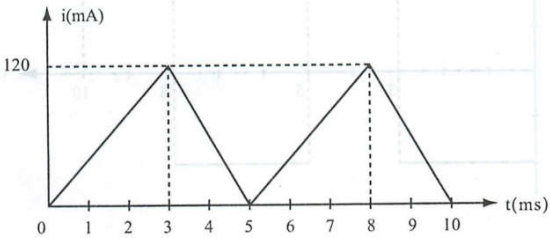
\includegraphics[scale=0.6]{pic1}
			\end{center}
			\begin{enumerate}[k]
				\item សរសេរកន្សោមកម្លាំងអគ្គិសនីចលករអាំងឌ្វី។
				\item គណនាកម្លាំងអគ្គិសនីចលករអាំងឌ្វីក្នុងចន្លោះពេលនីមួយៗ។
				\item សង់ក្រាភិចតាងឲ្យបម្រែបម្រួលនៃ $e$ តាមពេល។
			\end{enumerate}
		\item សូលេណូអុីតមួយមានប្រវែង $l=1.0m$ មានអង្គត់ផ្ចិត $D=4.0cm$ និងមានចំនួនស្ពៀ $N=1000$ ។
		\begin{enumerate}[k]
			\item គណនាអាំងឌុចតង់នៃសូលេណូអុីត។
			\item  គេធ្វើឲ្យចរន្តប្រែប្រួល $i=5t+2$ ឆ្លងកាត់សូលេណូអុីត។ ចូរអ្នកសរសេរកន្សោមកម្លាំងអគ្គិសនីចលករអូតូអាំងឌ្វី ដែលកើតមានក្នុងសូលេណូអុីត។
		\end{enumerate}
		\item សូលេណូអុីតមានប្រវែង $l=1.0m$ មានស្ពៀ $N=1000$ និងផ្ទៃមុខកាត់ $A=\frac{100cm^2}{\pi}$។ 
		\begin{enumerate}[k]
			\item គណនាអាំងឌុចតង់នៃសូលេណូអុីត។
			\item គណនាភ្លុចផ្ទាល់ កាលណាអាំងតង់សុីតេចរន្ត $I=0.5A$ ឆ្លងកាត់។
			\item គណនាកម្លាំងអគ្គិសនីចលករអាំងឌ្វីដែលមានក្នុងសៀគ្វី កាលណាគេធ្វើឲ្យចរន្តថយចុះពី $0.5A$ ទៅសូន្យរយៈពេល $\frac{1}{100}s$។
		\end{enumerate}
	\item បូប៊ីនមួយមានអាំងឌុចតង់ $L=0.5H$ ឆ្លងកាត់ដោយចរន្តប្រែប្រួល $i$ ដែលមានអាំងតង់សុីតេ $i=2.0A$។ \\គណនាថាមពលម៉ាញេទិចនៃបូប៊ីន។\newpage
	\item បូប៊ីនមួយឆ្លងកាត់ដោយចរន្តប្រែប្រួលដែលមានអាំងតង់សុីតេ $i=5A$ បានស្តុកថាមពលម៉ាញេទិច $E_L=6.25\times10^{-3}J$។\\ គណនាអាំងឌុចតង់នៃបូប៊ីន។
	\item បូប៊ីនមួយមានអាំងឌុចតង់ $L=0.02H$ បានស្តុកថាមពលអេឡិចត្រុងម៉ាញេទិច $E_L=0.5mJ$។\\ គណនាអាំងតង់សុីតេចរន្តដែលឆ្លងកាត់បូប៊ីន។
	\begin{multicols}{2}
		\item បូប៊ីនមួយមានអាំងឌុចតង់ $L=1.0mH$ និងមានរេសុីស្តង់អាចចោលបាន តជាសេរីនឹងអង្គធាតុចម្លងអូមដែលមានរេសុីស្តង់ $r=10.0\Omega$។ គេឲ្យចរន្តប្រែប្រួល $i=2t^2+5t$ ឆ្លងកាត់បូប៊ីននោះ។ \\ចូរសរសេរកន្សោមតង់ស្យុងរវាងគោលទាំងពីរនៃកំណាត់សៀគ្វីនោះ។
		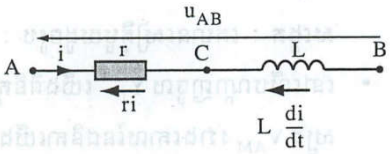
\includegraphics[scale=0.6]{pic03}
	\end{multicols}
	\item បូប៊ីនមួយមានរេសុីស្តង់ $R=5.0\Omega$ មានអាំងឌុចតង់ $L=5\times10^{-3}H$ ឆ្លងកាត់ដោយចរន្តប្រែប្រួល $i=5\sin314t$។\\
	ចូរសរសេរកន្សោមតង់ស្យុងរវាងគោលនៃបូប៊ីនជាអនុគមន៍នៃ $t$។
	\item បូប៊ីនមួយមានអាំងឌុចតង់ $L=500mH$ មានរេសុីស្តង់ $R=10.0\Omega$។ គណនាថេរពេលនៃបូប៊ីន។
	\begin{multicols}{2}
		\item តាមក្រាភិចចូរកំណត់៖
		\begin{enumerate}[k]
			\item ថេរពេលនៃឌីប៉ូល $\left(R,L\right)$។
			\item តម្លៃនៃអាំងឌុចតង់ $L$ បើគេដឹងថា $R=2.0\Omega$។
		\end{enumerate}
		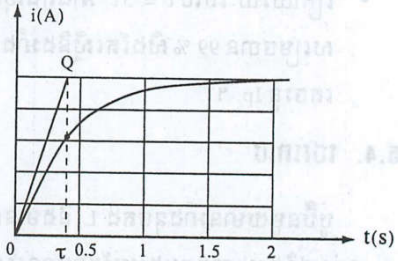
\includegraphics[scale=0.6, angle=1.0]{pic04}
	\end{multicols}
	\item កុងដង់សាទ័រមួយមានគោល $A$ និង $B$ មានកាប៉ាសុីតេ $C=22\mu F$ ផ្ទុកក្រោមតង់ស្យុង $V=E=4V$ បានភ្ជាប់ទៅនឹងគោល $M$ និង $N$ នៃបូប៊ីនមួយដែលមានអាំងឌុចតង់ $L=10mH$ និងមានរេសុីស្តង់អាចចោលបានដូចរូប៖
	\begin{multicols}{2}
		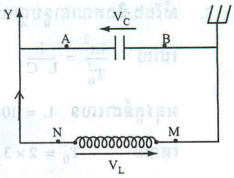
\includegraphics[scale=0.8]{pic02}
		\begin{enumerate}[k]
			\item ចូរបង្កើតសមីការឌីផេរ៉ង់ស្យែលនៃតង់ស្យុង $V_C$ ពេលដែលមានលំយោលអគ្គិសនី។
			\item ចូរអ្នកផ្ទៀងផ្ទាត់ថាអនុគមន៍៖
			$V_C=V_m\cos\left(\frac{2\pi}{T_0}t+\varphi_0\right)$ ជាចម្លើយនៃសមីការនោះ។
			\item សម្ដែង និងគណនាខួបផ្ទាល់ $T_0$ នៃលំយោលអគ្គិសនី។
			\item គណនាទំហំ $V_m$ និង $\varphi_0$។
		\end{enumerate}
	\end{multicols}
	\item នៅក្នុងសៀគ្វី $\left(L, C\right)$​មួយដែលមានរេសុីស្តង់អាចចោលបាន តង់ស្យុងរវាងគោលនៃកុងដង់សាទ័រមានតម្លៃ $V_1=250V$ កាលណាអាំងតង់សុីតេចរន្តក្នុងបូប៊ីនស្មើសូន្យ។\\
	គណនាអាំងតង់សុីតេចរន្ត កាលណាតង់ស្យុងរវាងគោលនៃកុងដង់សាទ័រស្មើ $100V$ ។ គេឲ្យកាប៉ាសុីតេនៃកុងដង់សាទ័រ $C=0.5\mu F$ និងអាំងឌុចតង់នៃបូប៊ីន $L=0.2H$។
	\item គណនាអាំងឌុចស្យុងនៃសូលេណូអុីតមួយដែលមានប្រវែង $l=40.0cm$ មានមុខកាត់ $A=20.0cm^2$ ហើយមានចំនួនស្ពៀ $N=1000$។ ចម្លើយ​: \fbox{$L=6.28mH$}
	\item គេចង់សង់បូប៊ីនមួយដែលមានរេសុីស្តង់ និងអាំងឌុចតង់ គេយកខ្សែចម្លងដែលមានកម្រាស់អុីសូឡង់អាចចោលបានទៅរុំលើសុីឡាំងអុីសូឡង់មួយមានប្រវែង $l=40.0cm$ មានអង្កត់ផ្ចិត $D=10.0cm$ ជា​​ស្ពៀ​​ជាប់ៗគ្នាចំនួនពីរជាន់ដែលក្នុងមួយជាន់មានស្ពៀ$500$។
	\begin{enumerate}[k]
		\item គណនារេសុីស្តង់ $R$ នៃបូប៊ីន បើខ្សែចម្លងនោះមានរេសុីស្ទីវីតេ $\rho=1.6\times10^{-8}\Omega\cdot m$។ ចម្លើយ​: \fbox{$R=10\Omega$}
		\item គណនាអាំងឌុចតង់នៃបូប៊ីន។ចម្លើយ​: \fbox{$L=25mH$}
	\end{enumerate}
	\item បូប៊ីនមួយអាចចាត់ទុកថាជាសូលេណូអុីតទ្រឹស្តី ដែលមានផ្ទៃមុខកាត់ $A=200.0cm^2$ មាន $n=1000$ ស្ពៀក្នុងមួយម៉ែត្រ និងមានប្រវែង $l=50.0cm$ ។
	\begin{enumerate}[k]
		\item គណនាអាំងឌុចតង់នៃបូប៊ីន។ ចម្លើយ​: \fbox{$L=12.6mH$}
		\item គណនាកម្លាំងអគ្គិសនីចលករអូតូអាំងឌ្វីដែលកើតមានក្នុងបូប៊ីន បើគេធ្វើឲ្យអាំងតង់សុីតេចរន្តប្រែប្រួលពី $0$ ទៅ $10.0A$ ក្នុងរយៈពេល $5s$។ ចម្លើយ​: \fbox{$e=25mV$}
		\item រកកន្សោមកម្លាំងអគ្គិសនីចលករអូតូអាំងឌ្ចី បើគេធ្វើឲ្យចរន្តឆ្លាស់ឆ្លងកាត់បូប៊ីនដែលមានសមីការ $i=I_m\sin\left(\omega t\right)$ ។\\
		ចម្លើយ​: \fbox{$e=-305\cos\left(1000\pi t\right)$}
		គេឲ្យ៖ $I_m=10.0A$ និង $\omega=1000\pi=3.14\times10^{3}rd\cdot s^{-1}$
	\end{enumerate}
	\item សូលេណូអុីតមួយមានអាំងឌុចតង់ $L=0.1H$។
	\begin{enumerate}[k]
		\item ចូរអ្នកឲ្យកន្សោមកម្លាំងអគ្គិសនីចលករអូតូអាំងឌ្វីដែលកើតមាន កាលណនាគេធ្វើឲ្យចរន្ត $i=3t^2$ ឆ្លងកាត់បូប៊ីន។ ចម្លើយ​: \fbox{$e=0.6t$}
		\item តើតម្លៃនៃកម្លាំងអគ្គិសនីចលករនោះស្មើប៉ុន្មាន នៅខណៈ $t_1=1.0s$ និង​ $t_2=10.0s$។ ចម្លើយ​: \fbox{$|e_1|=0.6V~,~|e_2|=6.0V$}
	\end{enumerate}
	\item \begin{enumerate}[k]
		\item គេផ្ទុកកុងដង់សាទ័រមួយដែលមានកាប៉ាសុីតេ $C=1\mu F$ ក្រោមតង់ស្យុង $V=E=2V$។\\
		គណនាថាមពលដែលស្តុកក្នុងកុងដង់សាទ័រនៅពេលផ្ទុក។
		\item កុងដង់សាទ័រដែលផ្ទុករួចនោះ បានតភ្ជាប់ទៅនឹងគោលនៃបូប៊ីនមួយដែលមានអាំងឌុចតង់ $L=0.1H$ និងមានរេសុីស្តង់អាចចោលបាន។ គណនាអាំងតង់សុីតេចរន្តអតិបរមា $i_m$។
	\end{enumerate}
	\item បូប៊ីនមួយមានរេសុីស្តង់ $R= 6.0\Omega$ និងមានអាំងឌុចតង់ $L$។
	\begin{enumerate}[k]
		\item គណនាអាំងឌុចតង់ $L$ បើថេរពេលមានតម្លៃ $\tau=2\times10^{-3}s$ ។ ចម្លើយ​: \fbox{$L=12\times10^{-3}H$}
		\item បូប៊ីននោះមានប្រវែង $l=30.0m$​មានចំនួនស្ពៀ $N=1000$។ គណនាអង្កត់ផ្ចិតនៃបូប៊ីន។ ចម្លើយ​: \fbox{$D=6cm$}
		\item គេធ្វើឲ្យចរន្តប្រែប្រួល $i=2t$ ឆ្លងកាត់បូប៊ីន។\\
		រកកន្សោមតង់ស្យុងរវាងគោលនៃបូប៊ីន។ ចម្លើយ​: \fbox{$V(t)=12t+0.024\left(V\right)$}
	\end{enumerate}
	\end{enumerate}
\borderline{ចប់}\\
\begin{center}
	\sffamily\color{blue}
	សូមសំណាងល្អ!
\end{center}\newpage
\end{document}